
\subsubsection{BLE フィンガープリントを用いた初期進行方向の補正}
% TODO:2. FPなのかフィンガープリントなのか統一した方がいいかも

BLEビーコンの基地局の位置情報を用いた補正手法は効果的である一方,基地局の
正確な位置情報を得るのが困難な場合がある.このような状況に対応するため,
本ライブラリではフィンガープリント(FP)を用いた補正手法も提供している.
この手法は,BLECorrectorクラスのFP機能として実装されている.

この手法を利用するために必要な情報は2つある.1つ目は前節と同様の
歩行者が移動中に収集したBLEビーコンのスキャンデータである.2つ目は
フィンガープリントデータである.これは事前に環境内の様々な位置で
計測された各ビーコンのID,電波強度,およびその計測位置の座標が
記録されたデータベースである.重要な点として,この手法では基地局の
正確な位置情報は必要としない.

この手法の利用例を以下に示す:


% TODO:3 BLECorrectorが被ってるのでキャプション名を変更した方がいいかも
\begin{lstlisting}[caption={BLECorrectorの使用例},label=lst:rotate-trajectory-using-ble-fingerprint,float=ht]
# フィンガープリントデータ
fingerprints = pd.read_csv('fingerprints.csv')
# ts: 1234567890.123  # 計測時刻(秒)
# x: 15.2            # 計測位置のx座標(メートル)
# y: 24.8            # 計測位置のy座標(メートル)
# bdaddress: "f2:65:d1:87:a4:2c"  # ビーコンID
# rssi: -68          # 電波強度(dBm)
# floor: "floor_5"   # フロア名

# BLECorrectorの初期化と補正の実行
corrector = BLECorrector(
    ble_realtime_scans=ble_scans,
    ble_fingerprints=fingerprints,
    rssi_threshold=-70
)
\end{lstlisting}


BLECorrectorのFPを用いた補正処理は,以下のように行われる.まず,
歩行者から受信した各BLE信号について,受信時刻$t$ごとに位置推定を行う.
各時刻において,受信したビーコンIDと同じデータポイントをFPデータベースから
抽出する.

各データポイントの重み$w$は,受信時刻$t$におけるRSSI値$r_t$と,
FPデータベース内の同じビーコンのRSSI値$r_f$との差に基づいて,
以下の式で計算される:

\begin{equation}
w_t = \exp\left(-\frac{(r_t - r_f)^2}{2\sigma^2}\right)
\end{equation}

ここで,$\sigma$は電波強度の標準偏差を表すパラメータであり,環境に応じて
調整可能である.この式はガウシアンカーネルに基づいており,RSSI値の差が
小さいほど大きな重みが与えられる.
% TODO:2.パスロスモデルの比重も増やせる説明をした方がいいかも

次に,これらの重みを用いて時刻$t$における推定位置$(p_x^t, p_y^t)$を
以下の式で計算する

\begin{equation}
p_x^t = \frac{\sum_{i=1}^{N_t} w_{t,i} x_i}{\sum_{i=1}^{N_t} w_{t,i}}, \quad
p_y^t = \frac{\sum_{i=1}^{N_t} w_{t,i} y_i}{\sum_{i=1}^{N_t} w_{t,i}}
\end{equation}

ここで,$(x_i, y_i)$はFPデータベース内の各データポイントの座標を表し,
$N_t$は時刻$t$において抽出されたデータポイントの総数である.この重み付き
平均により,その時刻のRSSI値と類似したデータポイントの座標がより強く
反映された推定位置が得られる.
% TODO:2.5 位置を推定した座標の図が欲しい
% TODO:2. 全体像を捉えて方向補正をするのが目的.なのでなんとなくこの辺にいそうというのが重要.
% 正確な位置を推定する必要はないといった方がいいかも

最適な回転角度の決定には,3.2.4節で導入した距離の総和$D(\theta)$を用いる.
ここでは,固定点として上記で推定された位置$(p_x^t, p_y^t)$を使用する.
最適な回転角度$\theta_{\mathrm{opt}}$は,前節と同様に距離の総和を
最小化する角度として決定される.

この手法の特徴は,基地局の正確な位置情報を必要としない点である.
その代わりに,事前に環境内で十分なFPデータを収集する必要があるが,
これは一度収集すれば継続的に使用できる.また環境の変化に応じて
FPデータを更新すれば,補正の精度を維持できる.


TODO:2 この図を入れるなら何かしらの説明がいる.同じ初期進行方向補正だから図はいらない気がする
% \begin{figure}[H]
%     \centering
%     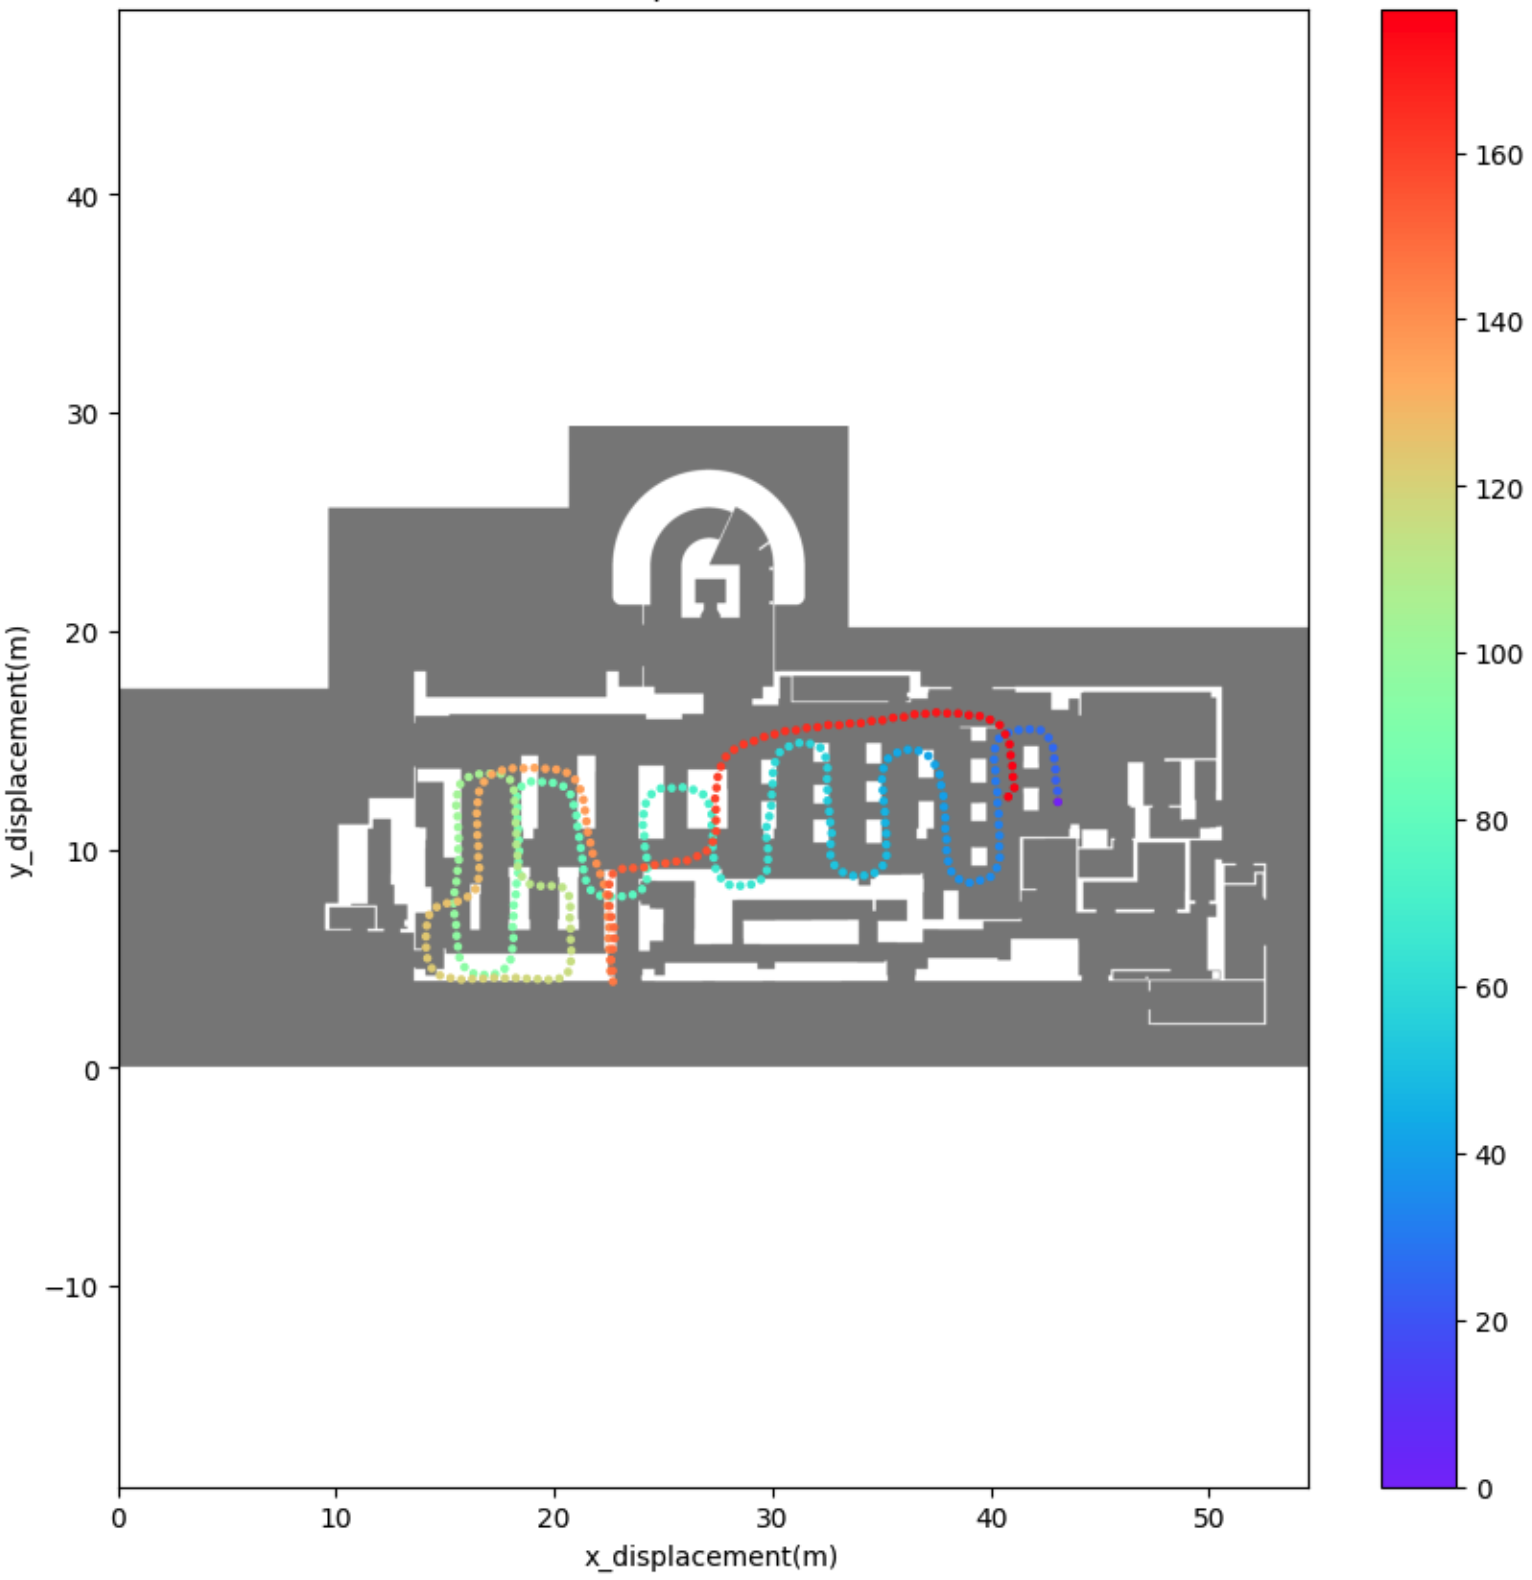
\includegraphics[width=\linewidth]{image/fingerprint-rotate.jpg}
%     \caption{BLEのFPを用いた補正後の軌跡}    \label{fig:fingerprint-rotate}
% \end{figure}

% TODO:2. 軌跡全体をみて最適化する形式だから十分なFPデータがなくても成り立つ

